\section{Thread Pools}

Downsides of using many threads include
\begin{itemize}
    \item longer time intervals before the same thread is scheduled again
    \item start and termination of threads has some overhead
    \item number of possible threads is limited
    \item Memory cost: Single stack for each thread
    \item full register-backup at preemption
\end{itemize}

A possible solution strategy is to allow for high parallelism in the problem space, but use a limited number of threads (\# threads \texttt{<=} \# processors).

\begin{description}
  \item[Tasks] define potentially parallel work packages that are \textit{independent} of each other.  
  \item[Task pool] Tasks are queued and executed by different worker threads. The number can be adapted to the system. Any task must complete execution before its worker thread can start another task.
  \textit{Programs that are modeled using tasks will automatically run aster on parallel machines.}
  \item[Return Values] from tasks are packaged into their own object type. \texttt{Future} in Java, \texttt{Promise} in JavaScript, \texttt{Task} in .NET, will return the result once it is available.
  
  Starting a task returns a future value that can be waited on using a method call.
  \item[Worker Threads] are usually daemon threads in TPL and ForkJoinPool: application can stop before the tasks end.
\end{description}

Submitting a task into the pool will launch the task asynchronously. Accessing the result from a future value will block until the task is terminated.

\subsection{Java Fork Join Pool}

Use \texttt{submit()} for asynchronous execution, \texttt{invoke()} for blocking execution.

\begin{lstlisting}
  var threadPool = new ForkJoinPool(); // create new pool
  var default = ForkJoinPool.commonPool(); // default pool as singleton
  
  Future<Integer> future = threadPool.submit(() => {
    int value = ...; // some long calculation
    return value;
    })

    int result = future.get(); // blocking call
  \end{lstlisting}
  
  \begin{figure}
    \centering
    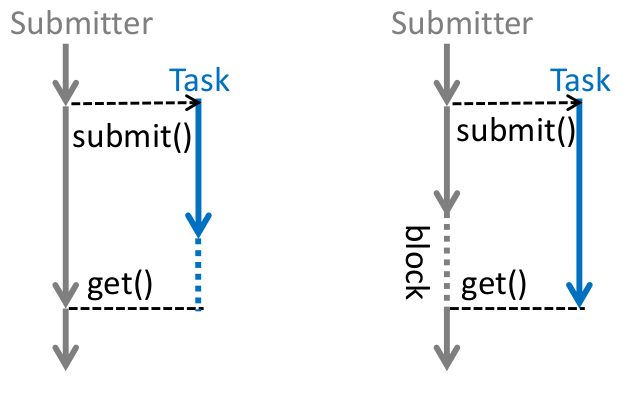
\includegraphics[width=6cm]{res/05-future.png}
    \caption{Future}
  \end{figure}

  \begin{description}
    \item[RecursiveAction] for tasks without return value (= \texttt{RecursiveTask<Void>})
    \item[invokeAll()] to start and wait for sub-tasks
  \end{description}

\subsection{.NET TPL: Task Parallel Library}
Has multiple abstraction layers:
\begin{itemize}
  \item Task Parallelization: use tasks explicitly
  \item Data Parallelization: use parallel statements and queries (implicit tasks)
  \item Asynchronous Programming (async/await)
\end{itemize}

\begin{description}
  \item[Exception in threads] terminates the program.
  \item[Fairness flag] not available.
  \item[Lock\&Condition] not available.
  \item[ReadWriteLockSlim] for upgradeable Read/Write Lock.
  \item[Semaphores] can be used at OS level.
  \item[Mutex] binary semaphore at OS level
  \item[Collections] are not thread safe, except \texttt{System.Collections.Concurrent} 
\end{description}

\begin{lstlisting}
  Task task = Task.Run(() => {
    // task implementation
  });
  // other code
  task.Wait(); // blocking call for task without return value
  Console.Write(task.Result); // blocking call, returns result
\end{lstlisting}

Nested tasks are possible:

\begin{lstlisting}
  var task = Task.Run(() => {
    var left = Task.Run(() => Count(leftPart));
    var right = Task.Run(() => Count(rightPart));
    return left.Result + right.Result;
  });
\end{lstlisting}

Using implicit Tasks, wait barrier at the end: \begin{lstlisting}
  Parallel.Invoke(
    () => MergeSort(l, m),
    () => MergeSort(m, r)
  );
\end{lstlisting}

Data Parallel for each:
\begin{lstlisting}
  Parallel.ForEach(list, 
    file => Convert(file)
  );
\end{lstlisting}


Data Parallel for (when iterations are independent):
\begin{lstlisting}
  Parallel.For(0, array.Length, 
    i => DoComputation(array[i])
  );
\end{lstlisting}

Parallel Loops will automatically group multiple iterations into one single task to avoid too much overhead.

\subsection{Parallel LINQ}

\begin{lstlisting}
  from book in bookCollection.AsParallel().AsOrdered()
    where book.Title.Contains("Concurrency")
    select book.ISBN
\end{lstlisting}

\subsection{Work Stealing}
In a work stealing scheduler, each processor in a computer system has a queue of work items (computational tasks, threads) to perform. 
Each work item consists of a series of instructions, to be executed sequentially, but in the course of its execution, a work item may also spawn new work items that can feasibly be executed in parallel with its other work. 
These new items are initially put on the queue of the processor executing the work item. 
When a processor runs out of work, it looks at the queues of the other processors and "steals" their work items. 
In effect, work stealing distributes the scheduling work over idle processors, and as long as all processors have work to do, no scheduling overhead occurs \href{https://en.wikipedia.org/wiki/Work\_stealing}{[1]}.